\subsubsection{QUBO, Hamiltonian, and Ising: Taxonomy}\label{sec:qubo-hamiltonian-ising-taxonomy}

At this point, several related concepts have been introduced:
\begin{itemize}
    \item QUBO (\autopageref{sec:qubo-problems})
    \item Hamiltonian (\autopageref{sec:hamiltonian-recap})
    \item Ising Model (only a brief introduction on the previous page)
\end{itemize}
Since they all involve energy functions and optimization, it is easy to confuse their roles. The purpose of this section is to clarify the relationship between them.

\highspace
\begin{flushleft}
    \textcolor{Green3}{\faIcon{search} \textbf{QUBO: The Optimization Problem}}
\end{flushleft}
A \textbf{Quadratic Unconstrained Binary Optimization (QUBO)} problem is a mathematical formulation used to describe optimization problems. It specifies:
\begin{equation*}
    \min_{x} E(x)
\end{equation*}
Where the variables are binary:
\begin{equation*}
    x_i \in \{0, 1\}
\end{equation*}
The QUBO itself does \textbf{not} describe a physical system. Instead, it describes the objective function that we want to optimize. Examples include: scheduling, portfolio optimization, routing, and resource allocation problems. Thus, QUBO belongs primarily to the world of \textbf{optimization theory}.

\highspace
\begin{flushleft}
    \textcolor{Green3}{\faIcon{bolt} \textbf{Hamiltonian: The Energy Operator}}
\end{flushleft}
A \textbf{Hamiltonian} is the mathematical object used in quantum mechanics to describe the energy of a physical system.

\highspace
For a quantum state \ket{\psi}, the Hamiltonian determines: the possible energy levels of the system, the time evolution of the system. Mathematically:
\begin{equation*}
    \hat{H}\ket{\psi_{i}} = E_i \ket{\psi_{i}}
\end{equation*}
The Hamiltonian therefore belongs to the world of \textbf{physics}.

\highspace
\begin{flushleft}
    \textcolor{Green3}{\faIcon{project-diagram} \textbf{Ising Model: A Particular Energy Formulation}}
\end{flushleft}
As we will see in the next section, the \textbf{Ising Model}, from the German physicist Ernst Ising, is a specific \emph{mathematical model} that was originally developed to describe magnetic materials.

\highspace
Instead of using binary variables:
\begin{equation*}
    x_{i} \in \{0, 1\}
\end{equation*}
It uses spin variables:
\begin{equation*}
    s_{i} \in \{-1, +1\}
\end{equation*}
The Ising Model provides a particular way of \textbf{writing the energy of a system as a function of the states of its spins}. In other words, the \hl{Ising model is a specific mathematical form for constructing Hamiltonians.}

\highspace
\begin{figure}[!htp]
    \centering
    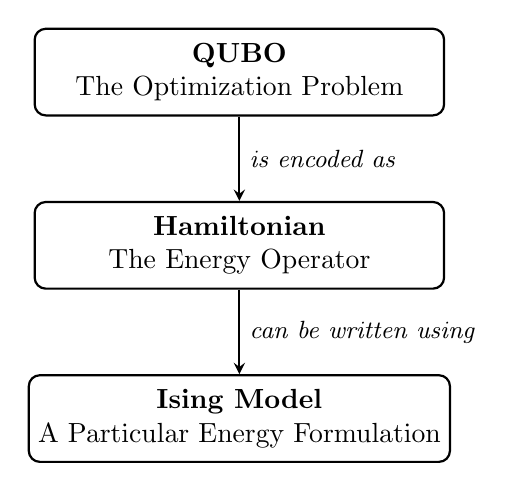
\begin{tikzpicture}[
        node distance=2.2cm,
        concept/.style={
            rectangle,
            rounded corners,
            draw=black,
            thick,
            minimum width=5.2cm,
            minimum height=1.1cm,
            align=center,
            font=\bfseries
        },
        relation/.style={
            ->,
            thick,
            >=stealth
        },
        label/.style={
            font=\small\itshape,
            midway,
            right,
            align=left
        }
    ]

        \node[concept] (qubo) {QUBO\\\normalfont The Optimization Problem};

        \node[concept, below of=qubo] (hamiltonian)
            {Hamiltonian\\\normalfont The Energy Operator};

        \node[concept, below of=hamiltonian] (ising)
            {Ising Model\\\normalfont A Particular Energy Formulation};

        \draw[relation] (qubo) -- node[label] {is encoded as} (hamiltonian);

        \draw[relation] (hamiltonian) -- node[label] {can be written using} (ising);

    \end{tikzpicture}
    \caption{Relationship between QUBO, Hamiltonian, and Ising model.}
\end{figure}

\highspace
\begin{flushleft}
    \textcolor{Red2}{\faIcon{question-circle} \textbf{We have already seen how to construct a Hamiltonian from a QUBO. So why do we need the Ising model?}}
\end{flushleft}
On \autopageref{sec:constructing-the-qubo-hamiltonian} we built a Hamiltonian directly from the QUBO energy landscape using projectors:
\begin{equation*}
    \hat{H} = \sum_{x \in \{0,1\}^{n}} E(x) \proj{x}
\end{equation*}
\textcolor{Green3}{\faIcon{check}} This was extremely useful for understanding the QUBO to Quantum Mechanics connection.

\highspace
\textcolor{Red2}{\faIcon{exclamation-triangle}} However, real \textbf{quantum annealers} (we will see them in the next sections) \textbf{do not directly implement arbitrary diagonal Hamiltonians}. Instead, they typically implement Hamiltonians based on the \textbf{Ising formulation}.

\highspace
\textcolor{Red2}{\faIcon{exclamation-triangle}} Furthermore, Hamiltonians are beautiful objects, even mathematically, but they are \textbf{not practical} for solving real-world problems. Let's imagine a problem with 100 variables, $n = 100$. Then, the Hamiltonian would be a $2^{100} \times 2^{100}$ matrix (because it acts on a Hilbert space of dimension $2^n$). This is an astronomically large matrix, and nature doesn't naturally give us a machine where we can say ``\emph{please implement this arbitrary diagonal matrix}''.

\highspace
Therefore, the next step is to \hl{study the Ising model} itself and \hl{understand how QUBO problems can be expressed using that formulation.}